\documentclass{beamer}

%% \documentclass[handout]{beamer}
%% % use this with the [handout] option to create handouts for the audience
%% \usepackage{pgfpages}
%% \pgfpagesuselayout{2 on 1}[a4paper,border shrink=5mm]

\mode<presentation>
{
  \usetheme{Diku}
% set this to your preferences:
  \setbeamercovered{invisible}
%  \setbeamercovered{transparent}
}

\usepackage{graphicx}
\usepackage{epic}

\usepackage{amsmath}
\usepackage{amssymb}
\usepackage{amsthm}

\newcommand{\basetop}[1]{\vtop{\vskip-1ex\hbox{#1}}}
\newcommand{\source}[1]{\let\thefootnote\relax\footnotetext{\scriptsize\textcolor{kugray1}{Source: #1}}}

% for coloured code citation in text:
\usepackage{fancyvrb}

%%%%%%%%%%%%%%%%%%%%%%%%%%%%%%%%%
%%%%%    code sections   %%%%%%%%
%%%%%%%%%%%%%%%%%%%%%%%%%%%%%%%%%

% code highlighting commands in own block
\DefineVerbatimEnvironment{code}{Verbatim}{fontsize=\scriptsize}
\DefineVerbatimEnvironment{icode}{Verbatim}{fontsize=\scriptsize}

% Fancy code with color commands:
\DefineVerbatimEnvironment{colorcode}%
        {Verbatim}{fontsize=\scriptsize,commandchars=\\\{\}}

%%%%%%%%%%%%%%%%%%%%%%%%%%%%%%%%%%
%%%%%    some coloring    %%%%%%%%

%% use "DIKU green" from our color theme for \emph
%\renewcommand{\emph}[1]{\textcolor{structure}{#1}}
%% use some not-too-bright red for an \emp command
%\definecolor{DikuRed}{RGB}{130,50,32}
%\newcommand{\emp}[1]{\textcolor{DikuRed}{ #1}}
%\definecolor{CosGreen}{RGB}{10,100,70}
%\newcommand{\emphh}[1]{\textcolor{CosGreen}{ #1}}


\definecolor{Red}{RGB}{220,50,10}
\definecolor{Blue}{RGB}{0,51,102}
\definecolor{Yellow}{RGB}{102,51,0}
\definecolor{Orange}{RGB}{178,36,36}
\definecolor{Grey}{RGB}{180,180,180}
\definecolor{Green}{RGB}{20,120,20}
\definecolor{Purple}{RGB}{160,50,100}
\newcommand{\red}[1]{\textcolor{Red}{{#1}}}
\newcommand{\blue}[1]{\textcolor{Blue}{{#1}}}
\newcommand{\yellow}[1]{\textcolor{Yellow}{{#1}}}
\newcommand{\orange}[1]{\textcolor{Orange}{{#1}}}
\newcommand{\grey}[1]{\textcolor{Grey}{{#1}}}
\newcommand{\green}[1]{\textcolor{Green}{{#1}}}
\newcommand{\purple}[1]{\textcolor{Purple}{{#1}}}




% use "DIKU green" from our color theme for \emph
\renewcommand{\emph}[1]{\textcolor{structure}{#1}}
% use some not-too-bright red for an \emp command
\definecolor{DikuRed}{RGB}{130,50,32}
\newcommand{\emp}[1]{\textcolor{DikuRed}{ #1}}
\definecolor{CosGreen}{RGB}{10,100,70}
\newcommand{\emphh}[1]{\textcolor{CosGreen}{ #1}}
\definecolor{CosBlue}{RGB}{55,111,122}
\newcommand{\emphb}[1]{\textcolor{CosBlue}{ #1}}
\definecolor{CosRed}{RGB}{253,1,1}
\newcommand{\empr}[1]{\textcolor{CosRed}{ #1}}

\newcommand{\mymath}[1]{$ #1 $}
\newcommand{\myindx}[1]{_{#1}}
\newcommand{\myindu}[1]{^{#1}}

\newtheorem{mydef}{Definition}
\newtheorem{mytheo}{Theorem}
\newtheorem{mylemma}{Lemma}

%%%%%%%%%%%%%%%%%%%%

\title[Intro]{Parallel Basic Blocks and\\ Flattening Nested Parallelism}

\author[C.~Oancea]{Cosmin E. Oancea and Troels Henriksen\\{\tt [cosmin.oancea,athas]@diku.dk}}

\institute{Department of Computer Science (DIKU)\\University of Copenhagen}


\date[Sept 2015]{September 2015 PMPH Lecture Notes}



\begin{document}

% \titleslide command WRAPS THIS SEQUENCE
%% % Set background to front page
%% \usebackgroundtemplate{
\includegraphics[width=\paperwidth,height=\paperheight]{front}}
%% {
%% \begin{frame}[plain]
%%   \titlepage
%% \end{frame}
%% }
\titleslide


\begin{frame}[fragile]
	\tableofcontents
\end{frame}

%%%%%%%%%%%%%%%%%%%%%%%%%%%%%%%%%%%%%%%
%%%%%%%% CONTENT STARTS HERE %%%%%%%%%%
%%%%%%%%%%%%%%%%%%%%%%%%%%%%%%%%%%%%%%%

\section{Homomorphisms (Continuation)}

\subsection{Almost Homomorphisms [Gorlatch'96]}

%\begin{frame}[fragile]
%	\tableofcontents[currentsubsection]
%\end{frame}

\begin{frame}[fragile,t]
  \frametitle{Almost Homomorphisms [Gorlatch]}

\emp{``Systematic Extraction and Implementation of Divide-and-Conquer Parallelism'', Sergei Gorlatch, 1996.} 
\bigskip

\emph{Intuition}: a non-homomorphic function $g$ can be sometimes ``lifted'' 
to a homomorphic one $f$, by computing a baggage of \emp{\em extra info}. 

\bigskip

The initial problem obtained by projecting the homomorphic result:\\
$g\mbox{ }=\pi\mbox{ }.\mbox{ }f$

\bigskip

\emp{Maximum-Segment Sum Problem ({\sc mss})}: \\
Given a list of integers, find the contiguous segment of the list 
whose members have the largest sum among all such segments.\\
The result is only the maximal sum (not the segment's members).

\bigskip

E.g., {\tt mss} [1, -2, 3, 4, -1, 5, -6, 1] = 11 \\
(the corresponding segment is [3, 4, -1, 5]). 

\end{frame}


\begin{frame}[fragile,t]
  \frametitle{Maximum Segment Sum}

\begin{block}{Incorrect list-homomorphism implementation}
\begin{colorcode}
mss []       = 0
mss (x{\tt ++}\mbox{ }y) = (mss x) \mymath{\uparrow} (mss y) -- \mymath{\uparrow} denotes Max
\end{colorcode}
\end{block} 

\smallskip

\alert{Incorrect:} {\tt (mss [1,-2,3,4])\mymath{\uparrow}(mss [-1,5,-6,1]) $\equiv$ 7 \mymath{\uparrow} 4 $\equiv$ 7} \\
\emph{The correct result} of {\tt (mss [1, -2, 3, 4, -1, 5, -6, 1])} \emph{is} 11, corresponding to segment [3, 4, -1, 5].

\bigskip

\emph{The segment of interest may lie partly in {\tt x} and partly in {\tt y}.} 
To construct a homomorphism we need to compute extra information:\pause
\begin{itemize}
    \item maximum concluding segment: {\tt mcs x = mcs [1,-2,3,4] = 7}
    \item maximum initial segment: {\tt mis y = mis [-1,5,-6,1] = 4}
    \item total segment sum: {\tt ts [1,-2,3,4] = 6}\pause
    \item {\tt mis (x++y) = (mis x) $\uparrow$ ((ts x)+(mis y))}, similar for {\tt mcs}    
    \item {\tt mss (x++y) = (mss x) $\uparrow$ (mss y) $\uparrow$ ((mcs x) + (mis y))}
\end{itemize}
\end{frame}


\begin{frame}[fragile,t]
  \frametitle{Maximum-Segment Sum = Near Homomorphism}

\begin{block}{Correct Solution -- Test it in Haskell!}
\begin{colorcode}
-- \mymath{x\mbox{ }\uparrow\mbox{ }y = if(x >= y) then x else y}
(mssx, misx, mcsx, tsx) \mymath{\odot} (mssy, misy, mcsy, tsy) = (
        (mssx\mymath{\mbox{ }\uparrow\mbox{ }}mssy\mymath{\mbox{ }\uparrow\mbox{ }}(mcsx+misy),
         misx\mymath{\mbox{ }\uparrow\mbox{ }}(tsx+misy),
        (mcsx+tsy)\mymath{\mbox{ }\uparrow\mbox{ }}mcsy,
         tsx + tsy
    )

f x = (x\mymath{\mbox{ }\uparrow\mbox{ }}0, x\mymath{\mbox{ }\uparrow\mbox{ }}0, x\mymath{\mbox{ }\uparrow\mbox{ }}0, x)

\emph{emss = (reduce \mymath{\odot} (0,0,0,0)) . (map f)}

\emp{mss  = \mymath{\pi\myindx{1}} . emss}
       where \mymath{\pi\myindx{1}} (a, _, _, _) = a 
\end{colorcode}
\end{block} 

\smallskip

The baggage: $3$ extra integers ({\tt misx, mcsx, tsx}) 
and a constant number of integer operations per communication stage. 

%Optimal time and work complexity with $N/log(N)$ processors.

\end{frame}


\begin{frame}[fragile,t]
  \frametitle{Longest Satisfying Segment Problems}

\begin{itemize}
    \item Class of problems which requires to find the longest segment of a list
            for which some property holds, for example:
    \item longest sequence of zeros, or longest sequence made from the same number, or longest sorted sequence.  
    \item How about longest sequence whose sum is 0?
    \item For the latter any correct solution needs to access the complete list, giving 
            sequential implementation without any parallelism, \\ e.g., {\tt lsum0 [4,1,1] $\odot$ lsum0[-2,5,1]}.
\end{itemize}

\bigskip

\begin{block}{Restrict the Shape of the Predicate:}
\begin{colorcode}
p []           = True
p [x]          = ...
p [x, y]       = ...
p [x : y : zs] = (p [x,y]) \mymath{\wedge} p (y : zs)
\end{colorcode}
\end{block} 

\end{frame}


\begin{frame}[fragile,t]
  \frametitle{Longest Satisfying Segment Problems}

\begin{block}{Restrict the Shape of the Predicate:}
\begin{colorcode}
zeroes [x]   = x == 0           same [x]   = True     sorted [x]   = True
zeroes [x,y] =  (zeroes [x])    same [x,y] = x == y   sorted [x,y] = x <= y
              \mymath{\wedge} (zeroes [y])
\end{colorcode}
\end{block} 

\bigskip
Extra Baggage:
\begin{itemize}
    \item As before, the \emp{length} of the longest initial/concluding  satisfying segments ({\tt lis}/{\tt lcs}),
            and the total list length ({\tt tl}).
    \item When considering the concatenation of the {\tt (lcs, lis)} pair, it is not guaranteed that the
            result satisfies the predicate \\
            e.g., {\tt (sorted x) $\wedge$ (sorted y) $\not\Rightarrow$ sorted x++y}.  
    \item Hence store the {\em last} element of {\tt lcs} and the {\em first} element of {\tt lis},
    \item and compute whether {\tt (lcs x)} is {\em connected} to {\tt (lis y)}, \\ i.e., {\tt p [lastx,firsty] == True}
    \item Boolean indicating whether the whole list satisfies {\tt p} ({\tt ok}).
\end{itemize}
\end{frame}

\begin{frame}[fragile,t]
  \frametitle{Longest Satisfying Segment Problem: Exercise}

\begin{block}{Exercise: fill in the blanks, test in Haskell for zeroes/same/sorted}
\begin{colorcode}
(lssx, lisx, lcsx, tlx, firstx, lastx, okx) \mymath{\odot}
(lssy, lisy, lcsy, tly, firsty, lasty, oky) 

  = (newlss, newlis, newlcs, tlx+tly, firstx, lasty, newok)
     where
        connect = ...
        newlss  = ...
        newlis  = ... 
        newlcs  = ... 
        newok   = ...

f x = (xmatch, xmatch, xmatch, 1, x, x, p [x])
    where xmatch = if (p [x]) then 1 else 0

\emph{elss = (reduce (\mymath{\odot}) (0,0,0,0,0,0,True)) . (map f)}

\emp{lss  = \mymath{\pi\myindx{1}} . elss}
       where \mymath{\pi\myindx{1}} (a, _, _, _, _, _, _) = a         
\end{colorcode}
\end{block} 

%lssx \mymath{\uparrow} lssy \mymath{\uparrow} (if connect then ... else 0)
%+ (if okx \mymath{\wedge} connect then ... else 0)
%+ (if oky \mymath{\wedge} connect then ... else 0)
%okx \mymath{\wedge} oky \mymath{\wedge} connect

\end{frame}



%\begin{frame}[fragile,t]
%  \frametitle{Longest Satisfying Segment Problem -- Solution}
%
%\begin{block}{Longest Satisfying Segment Solution}
%\begin{colorcode}
%(lssx, lisx, lcsx, tlx, firstx, lastx, okx) \mymath{\odot}
%(lssy, lisy, lcsy, tly, firsty, lasty, oky) 
%
%  = (newlss, newlis, newlcs, tlx+tly, firstx, lasty, newok)
%     where
%        connect = p [lastx, firsty]
%        newlss  = lssx \mymath{\uparrow} lssy \mymath{\uparrow} (if connect then lcsx+lisy else 0)
%        newlis  = lisx + (if okx \mymath{\wedge} connect then lisy else 0)
%        newlcs  = lcsy + (if oky \mymath{\wedge} connect then lcsx else 0)
%        newok   = okx \mymath{\wedge} oky \mymath{\wedge} connect
%
%f x = (xmatch, xmatch, xmatch, 1, x, x, p [x])
%    where xmatch = if (p [x]) then 1 else 0
%
%-- In Haskell write \emp{red \mymath{(\odot)\mbox{ }e\myindx{\odot}}}, where \mymath{e\myindx{\odot} = (0,0,0,0,0,0,True)}
%\emph{elss = (red \mymath{\odot}) . (map f)}
%
%\emp{lss  = \mymath{\pi\myindx{1}} . elss}
%       where \mymath{\pi\myindx{1}} (a, _, _, _, _, _, _) = a         
%\end{colorcode}
%\end{block} 
%
%\end{frame}

%%%%%%%%%%%%%%%%%%%%%%%%%%%%%%%%%%%%%%%
%%%%%%%%%%%%%%%%%%%%%%%%%%%%%%%%%%%%%%%
%%%%%%%%%%%%%%%%%%%%%%%%%%%%%%%%%%%%%%%
\subsection{Scan as a Distributable Homomorphism}
\begin{frame}[fragile]
	\tableofcontents[currentsubsection]
\end{frame}

\begin{frame}[fragile,t]
  \frametitle{All Homomorphism Are Efficient?}

If the combine operator involves concatenation then does
map-reduce provides efficient parallelization? 

\begin{block}{Merge Sort} \vspace{-1.5 ex}
\begin{columns}
\column{0.45\textwidth}
\begin{colorcode}[fontsize=\scriptsize]
-- merge two sorted lists
merge :: Ord T => [T] -> [T] -> [T]
merge [] y  = y
merge x  [] = x
merge (x:xs) (y:ys) = 
  if ( x <= y ) 
  then x : merge xs (y:ys)
  else y : merge (x:xs) ys 
\end{colorcode}
\column{0.45\textwidth}
\begin{colorcode}[fontsize=\scriptsize]
-- \emph{mSort} = \emp{hom merge [.] []}
-- [.] x = [x]  
\emph{mSort} :: Ord T => [T] -> [T]
\emph{mSort} []     = \emp{[]}
\emph{mSort} [x]    = \emp{[x]}
\emph{mSort} (x++y) = (\emph{mSort} x) \emp{`merge`}  
               (\emph{mSort} y)
\end{colorcode}
\end{columns}
\end{block}

In the naive merged sort, the {\tt merge} reduction operator
traverses sequentially the whole list, hence this map-reduce 
does not give efficient parallelization!

\end{frame}


\begin{frame}[fragile,t]
  \frametitle{Distributable Homomorphism (DH)}

\begin{itemize}
    \item DH: a class of homomorphisms that allows efficient parallel
            implem even if concatenation appears in the reduction operator.
    \item Requires that the length of the list is a power of 2,
            and at every step the list is split in half.
    \item {\tt zipWith :: [$\alpha$] $\rightarrow$ [$\beta$] $\rightarrow$ [$\gamma$]},\\
          {\tt zipWith $\odot$ [x$_1$,$\ldots$,x$_n$] [y$_1$,$\ldots$,y$_n$] $\equiv$ [x$_1\odot$y$_1$,$\ldots$,x$_n\odot$y$_n$]}
\end{itemize}
\vspace{-1ex}
\begin{mydef}[Distributable Homomorphism (DH)]\label{DistribHom}
Given two associative binary operators $\oplus$ and $\otimes$ we define operator \\
$\mbox{ }\mbox{ }\mbox{ }\mbox{ }$ 
{\tt dhop} ::  % (a$\rightarrow$a$\rightarrow$a) $\rightarrow$ (a$\rightarrow$a$\rightarrow$a) $\rightarrow$ 
                        [a] $\rightarrow$ [a] $\rightarrow$ [a] \\
$\mbox{ }\mbox{ }\mbox{ }\mbox{ }$ 
{\tt dhop}  u v = (zipWith $\oplus$ u v) ++ (zipWith $\otimes$ u v) \\  % $\oplus$ $\otimes$
\vspace{1ex}
We write $\oplus\updownarrow\otimes$ for the LH with combine operator {\tt dhop} $\oplus$ $\otimes$\\
$\mbox{ }\mbox{ }\mbox{ }\mbox{ }$ 
$\oplus\updownarrow\otimes$ [a]   $\mbox{ }\mbox{ }\mbox{ }\mbox{ }\mbox{ }\mbox{ }$    = [a] \\
$\mbox{ }\mbox{ }\mbox{ }\mbox{ }$ 
$\oplus\updownarrow\otimes$ (x ++ y) = ($\oplus\updownarrow\otimes$ x) {\tt `dhop`} ($\oplus\updownarrow\otimes$ y) \\
\vspace{1ex}
Function $h :: [T] -> [T]$ is a distributable homomorphism iff $h = \oplus\updownarrow\otimes$ for some binary associative
operators  $\oplus$ and $\otimes$.
\end{mydef}

\end{frame}


\begin{frame}[fragile,t]
  \frametitle{Distributed Reduce is a DH}

\begin{columns}
\column{0.4\textwidth}
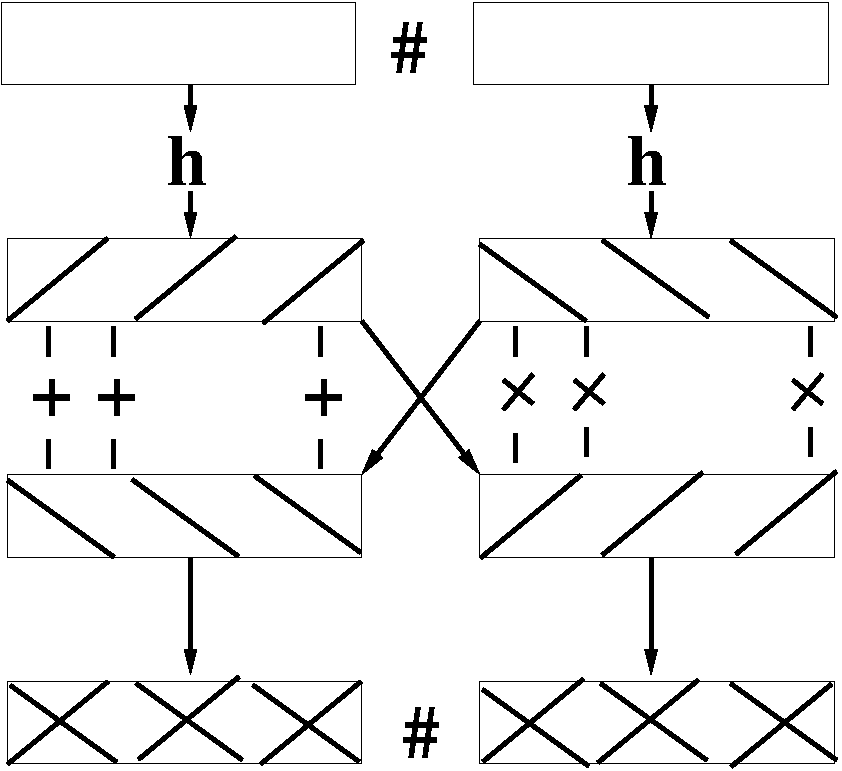
\includegraphics[height=25ex]{Figures/L2/DH}
\column{0.6\textwidth}\vspace{-3ex}
\begin{itemize}
    \item {\tt dhop u v = (zipWith $\oplus$ u v) ++}\\ 
          {\tt~~~~~~~~~~~(zipWith $\otimes$ u v)}
    \item {\tt $\oplus\updownarrow\otimes$ (x ++ y) = ($\oplus\updownarrow\otimes$ x)}\\
          {\tt~~~~~~~~~~`dhop` ($\oplus\updownarrow\otimes$ y)} 
\end{itemize}
\end{columns}

\begin{itemize}
    \item For example, distributed reduction: 
        {\tt distrRed ($\odot$) e$_\odot$ x = }\\
        {\tt [reduce $\odot$ e$_{\odot}$ x,$\ldots$, reduce $\odot$ e$_{\odot}$ x]}
    \item is a DH: distrRed $\odot$ = $\odot\updownarrow\odot$
\end{itemize}

\end{frame}


\begin{frame}[fragile,t]
  \frametitle{Scan is a DH}

\begin{columns}
\column{0.4\textwidth}
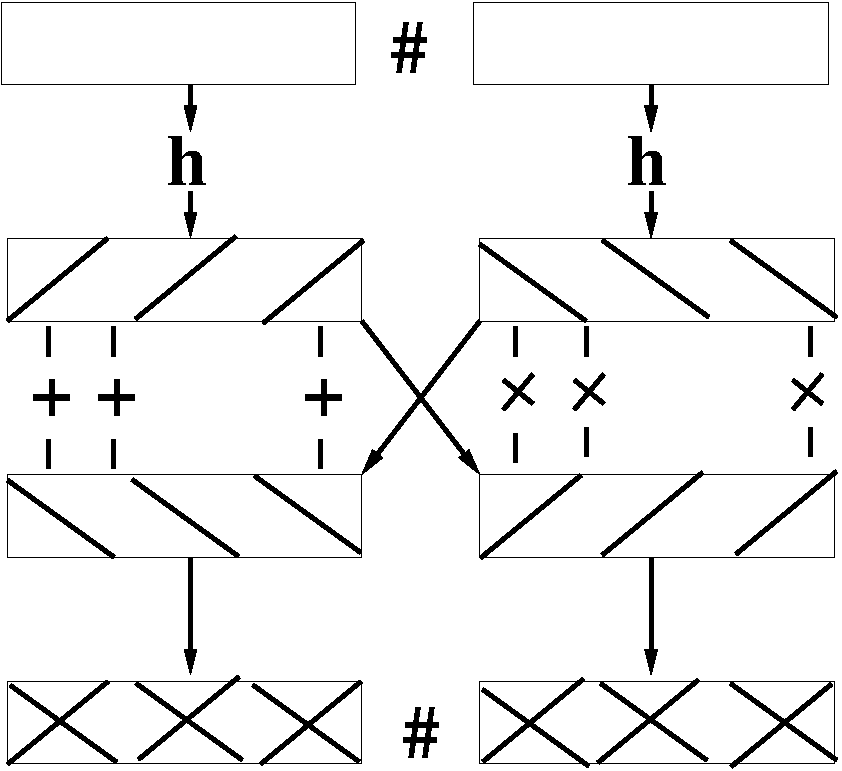
\includegraphics[height=25ex]{Figures/L2/DH}
\column{0.6\textwidth}\vspace{-3ex}
\begin{itemize}
    \item {\tt dhop u v = (zipWith $\oplus$ u v) ++}\\ 
          {\tt~~~~~~~~~~~(zipWith $\otimes$ u v)}
    \item {\tt $\oplus\updownarrow\otimes$ (x ++ y) = ($\oplus\updownarrow\otimes$ x)}\\
          {\tt~~~~~~~~~~`dhop` ($\oplus\updownarrow\otimes$ y)} 
    \item \alert{This implementation of scan is not work efficient,
                i.e., work $O(N \ lg \ N)$!}
\end{itemize}
\end{columns}


\begin{itemize}
    \item ${\tt scan} \ \odot \ {\tt e}_{\odot} \ {\tt(x++y)} = S_1~\oslash~S_2~=~S_1$
            {\tt ++ (map ($\odot$ s) $S_2$)},\\ 
            where $S_1${\tt = scan $\odot$ e$_{\odot}$ x},
                  $S_2${\tt = scan $\odot$ e$_{\odot}$ y}, and {\tt s=last $S_1$}\medskip
 
    \item {\tt dhScan $\odot$ e$_{\odot}$ = (map $\pi_1$) . ($\oplus\updownarrow\otimes$) . (map pair)},\\
            where {\tt $\pi_1$ (a,b) = a,~~~~pair a = (a,a)},\\
            {\tt (s$_1$,r$_1$) $\oplus$ (s$_2$,r$_2$) = (\alert{?}, \alert{?})}\\
            {\tt (s$_1$,r$_1$) $\otimes$ (s$_2$,r$_2$) = (\alert{?}, \alert{?})}
\end{itemize}

\end{frame}


\begin{frame}[fragile,t]
  \frametitle{Scan is a DH}

\begin{columns}
\column{0.4\textwidth}
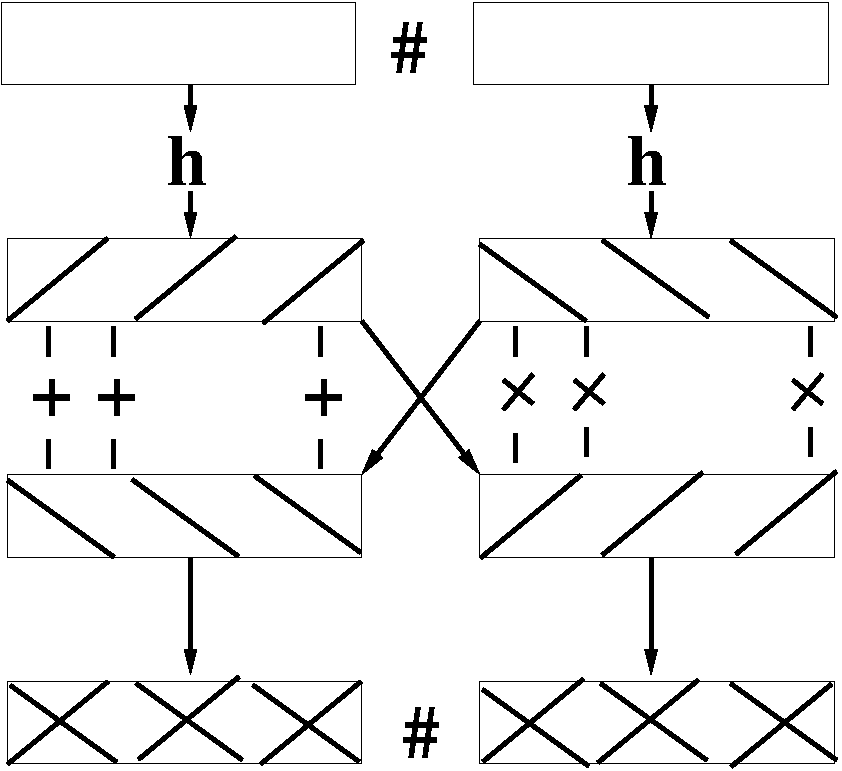
\includegraphics[height=25ex]{Figures/L2/DH}
\column{0.6\textwidth}\vspace{-3ex}
\begin{itemize}
    \item {\tt dhop u v = (zipWith $\oplus$ u v) ++}\\ 
          {\tt~~~~~~~~~~~(zipWith $\otimes$ u v)}
    \item {\tt $\oplus\updownarrow\otimes$ (x ++ y) = ($\oplus\updownarrow\otimes$ x)}\\
          {\tt~~~~~~~~~~`dhop` ($\oplus\updownarrow\otimes$ y)} 
    \item \alert{This implementation of scan is not work efficient,
                i.e., work $O(N \ lg \ N)$!}
\end{itemize}
\end{columns}


\begin{itemize}
    \item ${\tt scan} \ \odot \ {\tt e}_{\odot} \ {\tt(x++y)} = S_1~\oslash~S_2~=~S_1$
            {\tt ++ (map ($\odot$ s) $S_2$)},\\ 
            where $S_1${\tt = scan $\odot$ e$_{\odot}$ x},
                  $S_2${\tt = scan $\odot$ e$_{\odot}$ y}, and {\tt s=last $S_1$}\medskip
 
    \item {\tt dhScan $\odot$ e$_{\odot}$ = (map $\pi_1$) . ($\oplus\updownarrow\otimes$) . (map pair)},\\
            where {\tt $\pi_1$ (a,b) = a,~~~~pair a = (a,a)},\\
            {\tt (s$_1$,r$_1$) $\oplus$ (s$_2$,r$_2$) = (s$_1$, r$_1$ $\odot$ r$_2$)}\\
            {\tt (s$_1$,r$_1$) $\otimes$ (s$_2$,r$_2$) = (r$_1$ $\odot$ s$_2$, r$_1$ $\odot$ r$_2$)}
\end{itemize}

\end{frame}

%%%%%%%%%%%%%%%%%%%%%%%%%%%%%%%%%%%%%%%
%%%%%%%%%%%%%%%%%%%%%%%%%%%%%%%%%%%%%%%
%%%%%%%%%%%%%%%%%%%%%%%%%%%%%%%%%%%%%%%
\section{Implementation of Flat Bulk Operators}

\begin{frame}[fragile]
	\tableofcontents[currentsection]
\end{frame}

\subsection{Implementation of Reduce and Scan}

\begin{frame}[fragile,t]
  \frametitle{Parallel Random Access Machine (PRAM)}

PRAM focuses exclusively on parallelism and ignores issues
related to synchronization and communication:
\begin{itemize}
    \item[1] $p$ processors connected to shared memory
    \item[2] each processor has an unique id (index) $i$, $1 \leq i \leq p$
    \item[3] SIMD execution, each parallel instruction requires unit time,
    \item[4] each processor has a flag that controls whether it is active
                in the execution of an instruction.
\end  {itemize}


\begin{columns}
\column{0.6\textwidth}
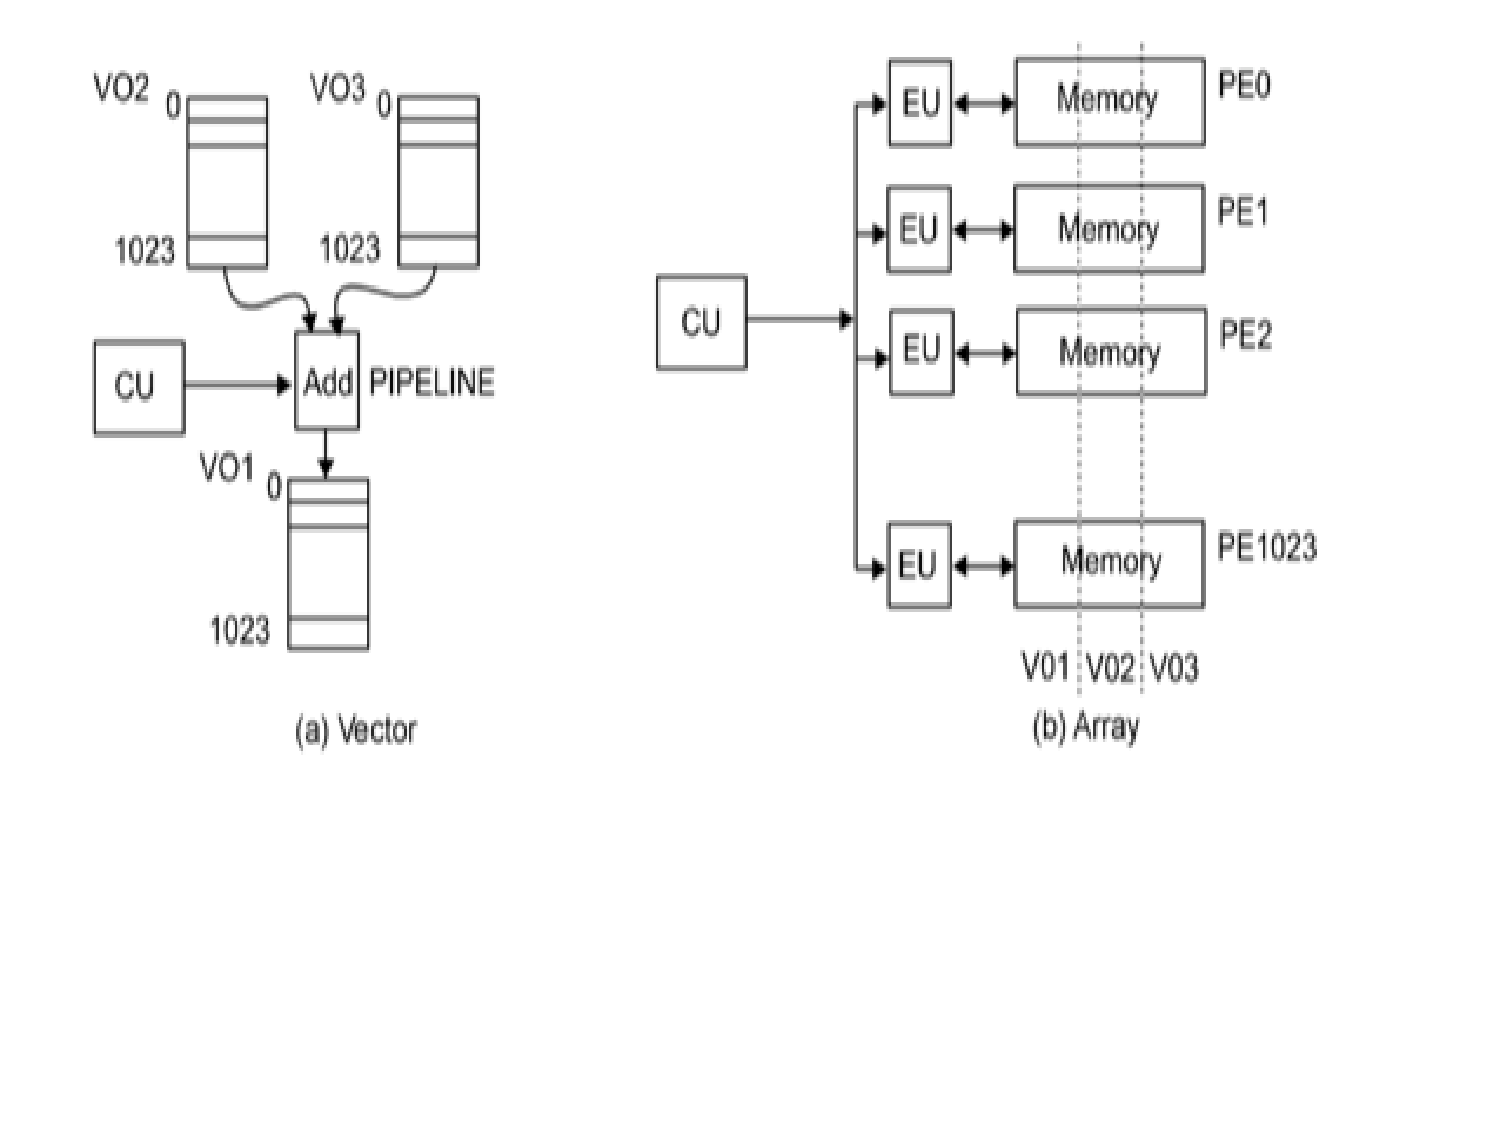
\includegraphics[height=37ex]{Figures/L2/VectorMachine}
\column{0.5\textwidth}\vspace{-15ex}
\begin{itemize}
    \item \emp{Work Time Algorithm (WT):}
    \item \emp{Work Complexity W(n)}: is the total \# of ops performed,
    \item \emp{Depth/Step Complexity D(n)}: is the \# of sequential steps.\medskip
    \item \emph{WT $\longrightarrow$ PRAM algorithm\\by Brent Theorem}.
\end{itemize}
\end{columns}

\end{frame}


\begin{frame}
  \frametitle{Reducing in Parallel}

\begin{columns}
\column{0.6\textwidth}
        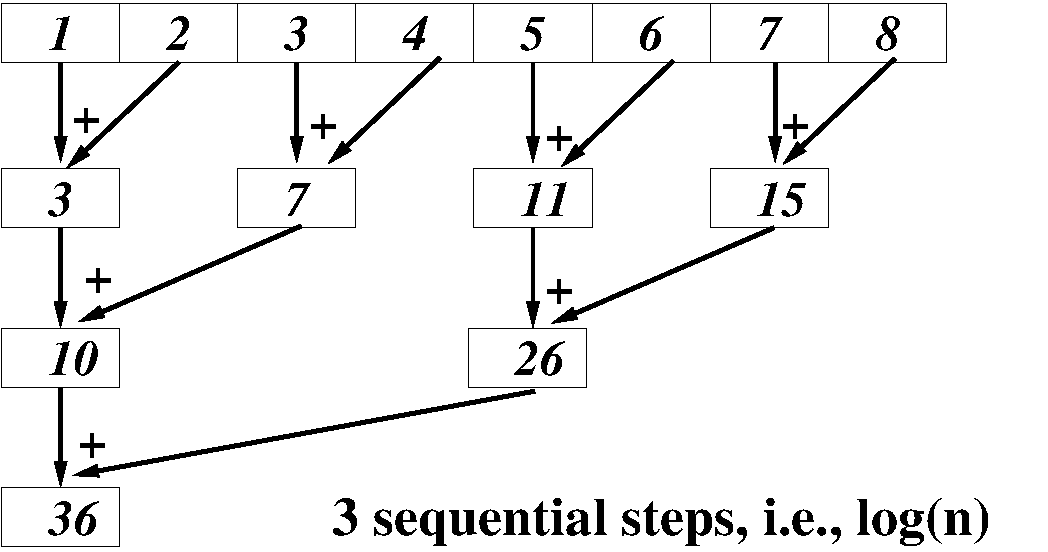
\includegraphics[height=22ex]{Figures/L2/ReduceEg.pdf} 
\column{0.5\textwidth}
Reducing an array of length {\tt n} with {\tt  n/2} processors requires:
\begin{itemize}
    \item work $W(n) = n$ and 
    \item depth $D(n) = lg \ n$, i.e., number of sequential steps.
    \item optimized runtime with $P$ processors: \emph{$(n/P) + lg \ P$.}
\end  {itemize}
\end{columns}

\begin{mytheo}[Brent Theorem]\label{BrentTh}
A Work-Time Algorithm of depth $D(n)$ and work $W(n)$ can be
simulated on a $P$-processor PRAM in time complexity T such that:\\\bigskip
\emp{$\ \ \ \ \ \ \ \ \ \ \ \ \ \ \ \ \frac{W(n)}{P} \leq T < \frac{W(n)}{P} + D(n)$}
\end{mytheo}

\end{frame}


\begin{frame}[fragile,t]
  \frametitle{Reduce: Algorithm and Complexity}


\begin{columns}
\column{0.5\textwidth}
\begin{colorcode}[fontsize=\scriptsize]
Input:  array A of n=2\mymath{\myindu{k}} elems of type T
        \mymath{\oplus::T\times T\rightarrow T} associative
Output: S = \mymath{\oplus\myindx{j=1}\myindu{n} a\myindx{j}}

1.  \emph{forall i = 0 to n-1 do}
2.    B[i] \mymath{\leftarrow} A[i]
3.  \emph{enddo}

4.  \emp{for h = 1 to k do}
5.    \emph{forall i = 0 to n-1 by 2\mymath{\myindu{h}} do} 
6.      B[i] \mymath{\leftarrow} B[i] \mymath{\oplus} B[i+2\mymath{\myindu{h-1}}]
7.    \emph{enddo}
8.  \emp{enddo}
9.  S \mymath{\leftarrow} B[0]  
\end{colorcode}
\column{0.59\textwidth}
\begin{itemize}
    \item $D_{1-3}(n) = \Theta(1)$, $W_{1-3}(n) = \Theta(n)$,
    \item $D_{5-7}(n) = \Theta(1)$, $W_{5-7}(n,h) = \Theta(n/2^h)$,
    \item $D_{4-8}(n) = k \times D_{5-7}(n) = \Theta(lg \ n)$
    \item $W_{4-8}(n) = \sum_{h=1}^k W_{5-7}(n,h) = $\\
          $\Theta(\sum_{h=1}^k (n/2^h) ) = \Theta(n)$
    \item $D_{9}(n) = \Theta(1)$, $W_{9}(n) = \Theta(1)$,\bigskip
    \item \emp{$D(n) = \Theta(lg \ n), W(n) = \Theta(n)$!}
\end{itemize}
\end{columns}
\bigskip

%\mymath{\frac{n}{2\myindu{h}}} do}

\begin{center}  
\emp{$\frac{n-1}{P} \leq  Runtime < \frac{n-1}{P} + lg \ n$}
\end{center}


\end{frame}


\begin{frame}[fragile,t]
  \frametitle{Parallel Exclusive Scan with Associative Operator $\oplus$}
\bigskip

\begin{columns}
\column{0.4\textwidth}
        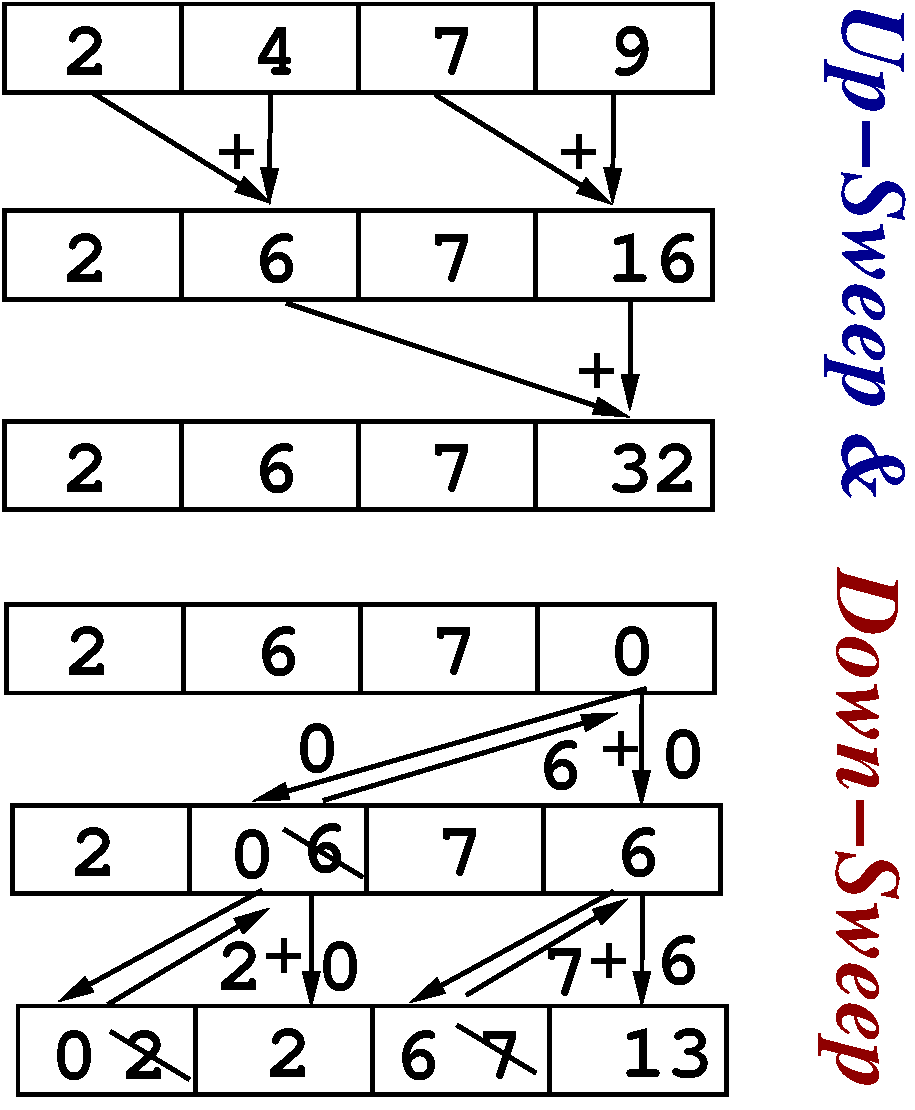
\includegraphics[height=33ex]{Figures/L2/ScanEg.pdf} 
\column{0.6\textwidth}
Two Steps:
\begin{itemize}
    \item \blue{Up-Sweep:} similar with reduction
    \item Root is replaced with neutral element.
    \item \emp{Down-Sweep:} 
    \begin{itemize}
        \item the left child sends its value to parent and 
                updates its value to that of parent.
        \item the right-child value is given by $\oplus$ 
                applied to the left-child value and
                the (old) value of parent.
        \item note that the right child is in fact the parent,
                i.e., in-place algorithm.
    \end  {itemize}
\end  {itemize}
\end{columns}


\end{frame}



\begin{frame}[fragile,t]
  \frametitle{Parallel Exclusive Scan Algorithm And Complexity}
\bigskip

\begin{columns}
\column{0.5\textwidth}
\begin{colorcode}[fontsize=\scriptsize]
Input:  array A of n=2\mymath{\myindu{k}} elems of type T
        \mymath{\oplus::T\times T\rightarrow T} associative
Output: B = \mymath{[0, a\myindx{1}, a\myindx{1}\oplus{}a\myindx{2},\ldots,\oplus\myindx{j=1}\myindu{n-1} a\myindx{j}]}

1.  \emph{forall i = 0 : n-1 do}
2.    B[i] \mymath{\leftarrow} A[i]
3.  \emph{enddo}

4.  \emp{for d = 0 to k-1 do} \emph{// up-sweep}
5.    \emph{forall i = 0 to n-1 by 2\mymath{\myindu{d+1}} do} 
6.      B[i+2\mymath{\myindu{d+1}}-1] \mymath{\leftarrow} B[i+2\mymath{\myindu{d}}  -1] \mymath{\oplus} 
                       B[i+2\mymath{\myindu{d+1}}-1]
7.    \emph{enddo}
8.  \emp{enddo}
9.  B[n-1] = 0
10. \emp{for d = k-1 downto 0 do} \emph{// down-sweep}
11.   \emph{forall i = 0 to n-1 by 2\mymath{\myindu{d+1}} do} 
12.     tmp \mymath{\leftarrow} B[i+2\mymath{\myindu{d}}-1]
13.     B[i+2\mymath{\myindu{d}}-1] \mymath{\leftarrow} B[i+2\mymath{\myindu{d+1}}-1]
14.     B[i+2\mymath{\myindu{d+1}}-1] \mymath{\leftarrow} tmp \mymath{\oplus} B[i+2\mymath{\myindu{d+1}}-1]
15.   \emph{enddo}
16. \emp{enddo}
\end{colorcode}
\column{0.59\textwidth}
\begin{itemize} 
    \item The code show exponentials for clarity, but those can
            be computed by one multiplication/division operation
            each sequential iteration.
    \item \emp{$D(n) = \Theta(lg \ n), W(n) = \Theta(n)$!}
    \item Similar reasoning as with reduce.
\end{itemize}
\end{columns}

%4.  \emp{for h = 1 to k do} // up-sweep
%5.    \emph{forall i \mymath{\in} n : 1 by -2\mymath{\myindu{h}} do} 
%6.      B[i] \mymath{\leftarrow} B[i] \mymath{\oplus} B[i-2\mymath{\myindu{h-1}}]
%7.    \emph{enddo}
%8.  \emp{enddo}
%9.  B[n] = 0
%
%10. \emp{for h = k downto 1 do} // down-sweep
%11.   \emph{forall i \mymath{\in} n : 1 by -2\mymath{\myindu{h}} do} 
%12.     tmp = B[i]
%13.     B[i] \mymath{\leftarrow} B[i] \mymath{\oplus} B[i-2\mymath{\myindu{h-1}}]
%14.     B[i-2\mymath{\myindu{h-1}}] = tmp
%15.   \emph{enddo}
%16. \emp{enddo}


\end{frame}

%%%%%%%%%%%%%%%%%%%%%%%%%%%%%%%%%%%%%%%%%
%%%%%%%%%%%%%%%%%%%%%%%%%%%%%%%%%%%%%%%%%
\subsection{Other Second-Order Bulk Operators}

\begin{frame}[fragile,t]
  \frametitle{Zip, ZipWith}

\begin{itemize}
    \item \emph{\tt zip :: [$T_1$] $\rightarrow$ [$T_2$] $\rightarrow$ [($T_1$,$T_2$)]}
    \item \emp{\tt zip [a$_1$,$\ldots$,a$_n$] [b$_1$,$\ldots$,b$_m$] $\equiv$ [(a$_1$,b$_1$),\ldots,(a$_q$,b$_q$)]},
            where {\tt q = min(m,n)}.
    \item \emph{\tt unzip :: [($T_1$,$T_2$)] $\rightarrow$ ([$T_1$],[$T_2$])}
    \item \emp{\tt unzip [(a$_1$,b$_1$),\ldots,(a$_n$,b$_n$)]$\equiv$([a$_1$,$\ldots$,a$_n$],[b$_1$,$\ldots$,b$_n$])},\medskip

    \item In some sense {\tt zip} is syntactic sugar, for example one could work with the
            tuple of array representation, e.g.,
    \item \emp{\tt mapT :: (($\alpha_1$,$\ldots$,$\alpha_m$)$\rightarrow$($\beta_1$,$\ldots$,$\beta_n$)) $\rightarrow$}\\ 
          \emp{\tt~~~~~~~~~[$\alpha_1$] $\rightarrow\ldots\rightarrow$ [$\alpha_m$] $\rightarrow$ ([$\beta_1$],$\ldots$,[$\beta_n$]])}
    \item \emph{\tt mapT f $\equiv$ unzip$^n$ . map f . zip$^n$}\medskip

    \item {\tt zipWith :: [$\alpha_1$] $\rightarrow$ [$\alpha_2$] $\rightarrow$ [$\beta$]}
    \item {\tt zipWith $\odot$ [a$_1$,$\ldots$,a$_n$] [b$_1$,$\ldots$,b$_n$] $\equiv$ [a$_1\odot$b$_1$,$\ldots$,a$_n\odot$b$_n$]}
    \item {\tt zipWith $\odot$ $\equiv$ map ($\backslash$(u,v) $\rightarrow$ u $\odot$ v) . zip}
\end  {itemize}

\end{frame}

\begin{frame}[fragile,t]
  \frametitle{Permute, Write, Split, Filter}

\begin{itemize}
    \item Operator to \emph{permute in parallel} based on a set (array) of indices:\\
          \emph{permute :: [Int] $\rightarrow$ [$\alpha$] $\rightarrow$ [$\alpha$]}, e.g.,\\
           A (data vector) {\tt~= [a0,~a1,~a2,~a3,~a4,~a5]}\\
           I (index vector){\tt~~= [3,~~2,~~0,~~4,~~1,~~5~]}\\
           \emp{permute I A     {\tt~~~~= [a2,~a4,~a1,~a0,~a3,~a5]}}\bigskip

    \item Operator to \emph{write in parallel} a set of values to 
            correspond indices:\\
          \emph{write :: [Int] $\rightarrow$ [$\alpha$] $\rightarrow$ [$\alpha$] $\rightarrow$ [$\alpha$]}\\
          A (data vector) {\tt~=[b0, b1, b2]}\\
          I (index vector){\tt~~=[2,~~4,~~1]}\\
          X (input array) {\tt~=[a0,~a1,~a2,~a3,~a4,~a5]}\\
          \emp{write I A X     {\tt~~~~=[a0,~b2,~b0,~a3,~b1,~a5]}}\bigskip

    \item %Operator to {\tt split} a list (array) at a certain index:\\
          \emph{\tt split :: Int $\rightarrow$ [$\alpha$] $\rightarrow$ ([$\alpha$],[$\alpha$])}\\
          \emp{\tt split i [a$_0$,$\ldots$,a$_n$] $\equiv$ ([a$_0$,$\ldots$,a$_{i-1}$], [a$_i$,$\ldots$,a$_{n}$])}\smallskip
    \item \emph{\tt replicate :: Int $\rightarrow$ $\alpha$ $\rightarrow$ [$\alpha$]}\\
            \emp{\tt replicate N a $\equiv$ [a, a,$\ldots$, a]}, i.e., {\tt a} is replicated {\tt N} times.  
 
\end  {itemize}

\end{frame}

\begin{frame}[fragile,t]
  \frametitle{Filter: Implementation based on Map and Scan}

%\mymath{\backslash}

\emph{\tt filter :: ($\alpha\rightarrow$Bool) $\rightarrow$ [$\alpha$] $\rightarrow$ [$\alpha$]}\\
Filters out the input-list elements that do NOT satisfy the predicate.
%\emp{\tt filter cond X $\equiv$ [b$_0$,$\ldots$,b$_{m}$]}, such that 
%{\tt b$_j, \forall j\in\{0\ldots m\}$,} are all the elements of array 
%{\tt X} that evaluate to {\tt True} under condition {\tt cond}, i.e., {\tt (cond b$_j$) $\equiv$ True}.\medskip

\alert{Can {\tt filter} be implemented via {\tt map} and {\tt reduce} (and {\tt scan})?}\pause


\begin{columns}
\column{0.59\textwidth}
\begin{colorcode}[fontsize=\scriptsize]
parFilter :: (a->Bool) -> [a] -> ([a], [Int])
parFilter cond X = 
let n   = length arr
    cs  = map cond X
    tfs = map (\mymath{\backslash}f->if f then 1 
                        else 0) cs
    isT = scan\mymath{\myindu{inc}} (+) 0 tfs
    i   = last isT

    ffs = map (\mymath{\backslash}f->if f then 0 
                        else 1) cs
    isF = (map (+ i) . scan\mymath{\myindu{inc}} (+) 0) ffs

    inds= map (\mymath{\backslash} (c,iT,iF) -> 
                  if c then iT-1 else iF-1 ) 
              (zip3 cs isT isF)
    flags = write [0,i] [i,n-i] (replicate n 0)
in  (permute X inds, flags)
\end{colorcode}
\column{0.4\textwidth}
\begin{colorcode}[fontsize=\scriptsize]
Assume X = [5,4,2,3,7,8], and 
cond is T(rue) for even nums.
n   = 6
cs  = [F, T, T, F, F, T]
tfs = [0, 1, 1, 0, 0, 1]

isT = [0, 1, 2, 2, 2, 3]
i   = 3

ffs = [1, 0, 0, 1, 1, 0]

isF = [4, 4, 4, 5, 6, 6]

inds= [3, 0, 1, 4, 5, 2]


flags  = [3, 0, 0, 3, 0, 0]
Result = [4, 2, 8, 5, 3, 7] 
\end{colorcode}
\end{columns}

\end{frame}

%%%%%%%%%%%%%%%%%%%%%%%%%%%%%%%%%%%%%%%%%%%%%
%%%%%%%%%%%%%%%%%%%%%%%%%%%%%%%%%%%%%%%%%%%%%
%%%%%%%%%%%%%%%%%%%%%%%%%%%%%%%%%%%%%%%%%%%%%

\section{Nested Data Parallelism and Flattening}

\begin{frame}[fragile]
	\tableofcontents[currentsection]
\end{frame}

\subsection{Segmented Scan}

\begin{frame}[fragile,t]
  \frametitle{Segmented Inclusive Scan with Operator $\oplus$}

\begin{columns}
\column{0.55\textwidth}
\begin{colorcode}
-- iota n = [0..n-1]
map (\mymath{\backslash}i-> scan (+) 0 [1..i]) [3,4] \emph{\mymath{\equiv}}
[ scan\mymath{\myindu{inc}} (+) 0 [1,2,3], 
  scan\mymath{\myindu{inc}} (+) 0 [1,2,3,4] ] 
      \emph{\mymath{\equiv}}
[ [1,3,6], [1,3,6,10] ]
\end{colorcode}
\column{0.55\textwidth}
\begin{colorcode}
-- \blue{Flags \& Flat Data Representation:}
sgmScanInc (+) 0 [1,0,0,1,0,0,0] -- \emph{flag}
                 [1,2,3,1,2,3,4] -- \emp{data}
    \emph{\mymath{\equiv}}
( [1,0,0,1,0,0, 0],              -- \emph{flag}
  [1,3,6,1,3,6,10] )             -- \emp{data}
\end{colorcode}
\end{columns}
\medskip

Can be obtained by replacing the following operator:
\smallskip

\begin{colorcode}
sgmScanInc :: (a->a->a) -> a -> [Int] -> [a] -> [a]
sgmScanInc \mymath{\odot} ne flags data = 
  let fds = zip flags data
      (_,r) = unzip \$ 
              scan\mymath{\myindu{inc}} (\mymath{\backslash}(f1,v1) (f2,v2) -> 
                        let f = f1 .|. f2  -- bitwise or
                        in  if f2 == 0
                            then (f, v1 \mymath{\odot} v2)
                            else (f, v2)
                     ) (0,ne) fvs
  in  r
\end{colorcode}
\bigskip

\alert{How about Exclusive Scan?}

\end{frame}

\begin{frame}[fragile,t]
  \frametitle{{\scriptsize Slide from CMU 15-418: Parallel Computer Architecture and Programming (Spring 2012)}}
\vspace{-3ex}
\begin{center}
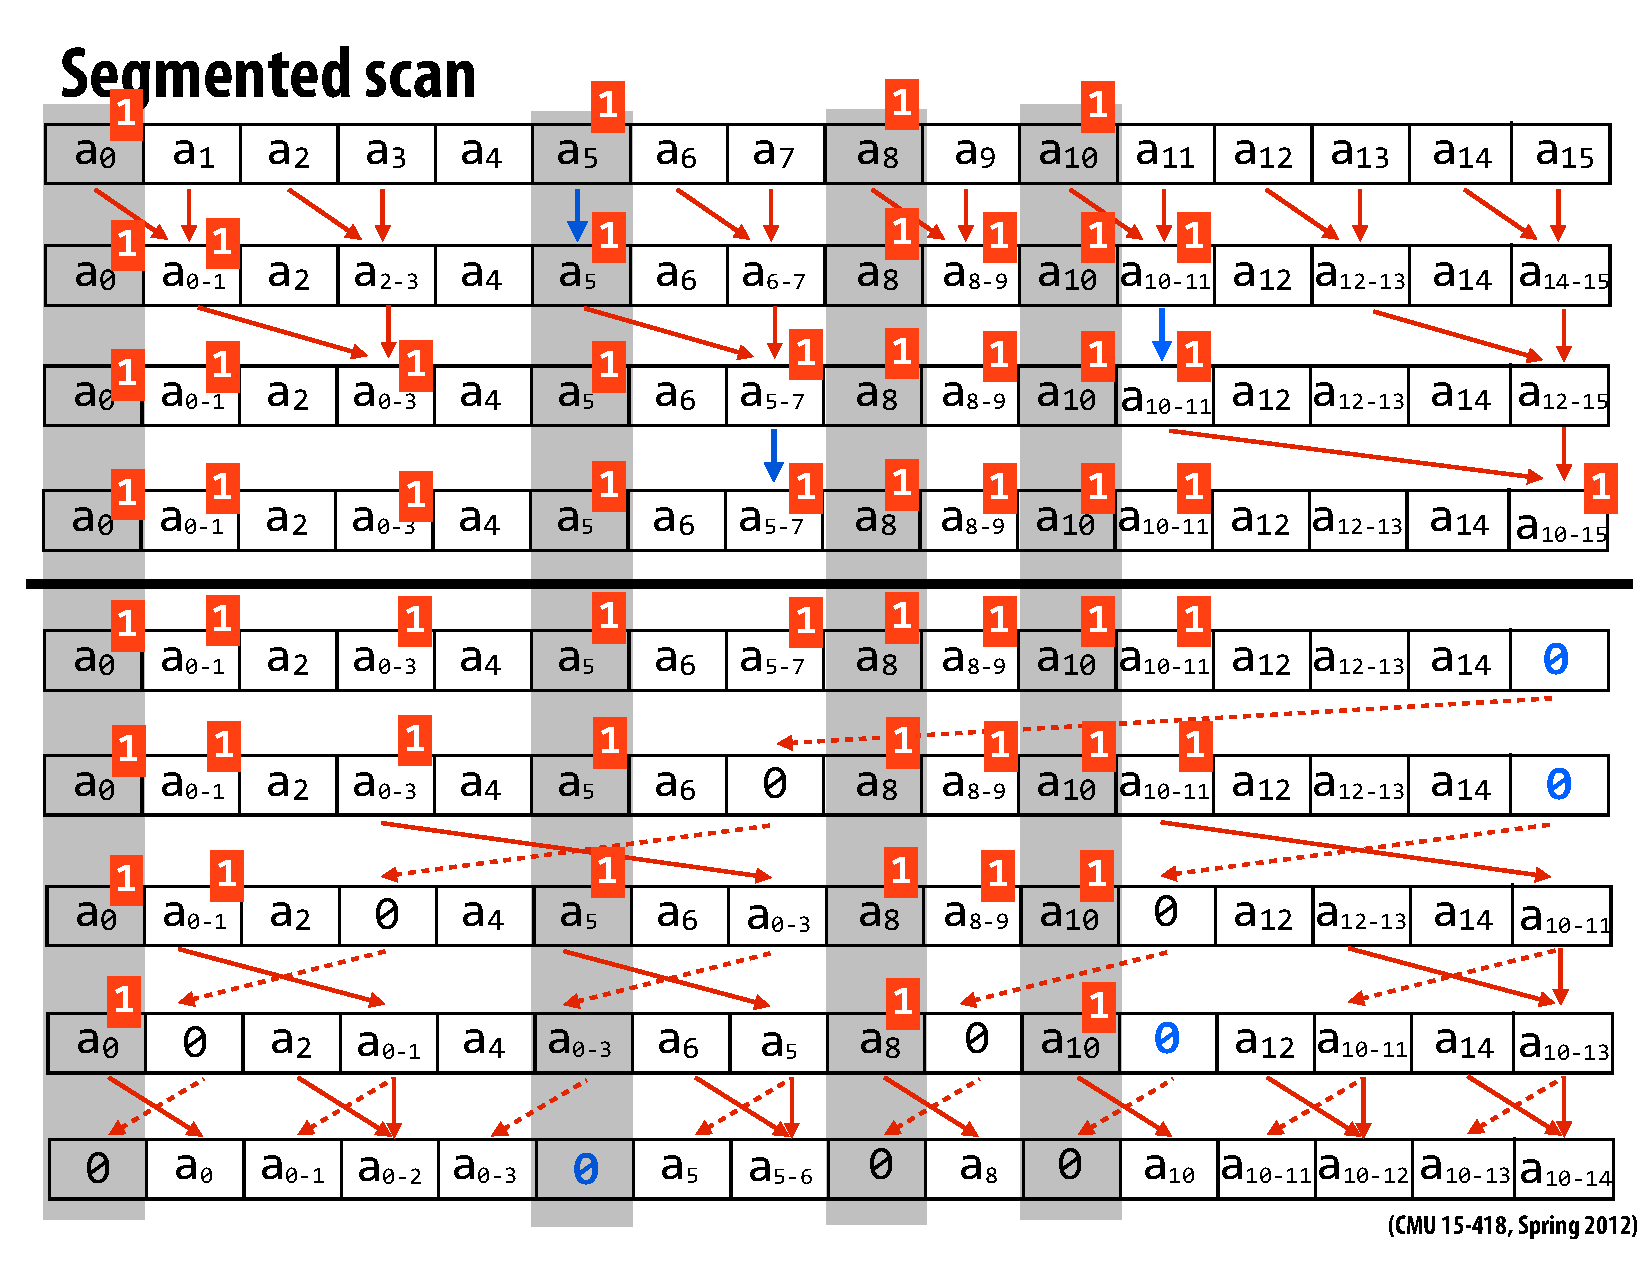
\includegraphics[height=50ex]{Figures/L2/SegmExclScan} 
\end  {center}

\end{frame}


\begin{frame}[fragile,t]
  \frametitle{Segmented Exclusive Scan Alg And Complexity}
\vspace{-2ex}
\begin{columns}
\column{0.6\textwidth}
\begin{colorcode}[fontsize=\scriptsize]
Input:  flag array F of n=2\mymath{\myindu{k}} of ints
        data array A of n=2\mymath{\myindu{k}} elems of type T
        \mymath{\oplus::T\times T\rightarrow T} associative
Output: B = segmented scan of 2-dim array A
1.  \emph{FORALL i = 0 to n-1 do} B[i] \mymath{\leftarrow} A[i] \emph{ENDDO}
2.  \emp{FOR d = 0 to k-1 DO} \emph{// up-sweep}
3.    \emph{FORALL i = 0 to n-1 by 2\mymath{\myindu{d+1}} DO} 
4.      IF F[i+2\mymath{\myindu{d+1}}-1] == 0 THEN 
5.          B[i+2\mymath{\myindu{d+1}}-1] \mymath{\leftarrow} B[i+2\mymath{\myindu{d}}-1] \mymath{\oplus} B[i+2\mymath{\myindu{d+1}}-1]
6.      ENDIF
7.      F[i+2\mymath{\myindu{d+1}}-1] \mymath{\leftarrow} F[i+2\mymath{\myindu{d}}-1] .|. F[i+2\mymath{\myindu{d+1}}-1]
8.  \emp{ENDDO} \emph{ENDDO}
9.  B[n-1] \mymath{\leftarrow} 0
10. \emp{FOR d = k-1 downto 0 DO} \emph{// down-sweep}
11.   \emph{FORALL i = 0 to n-1 by 2\mymath{\myindu{d+1}} DO} 
12.     tmp \mymath{\leftarrow} B[i+2\mymath{\myindu{d}}-1]
13.     IF \alert{F\_original}[i+2\mymath{\myindu{d}}] \mymath{\neq} 0 THEN
14.          B[i+2\mymath{\myindu{d+1}}-1] \mymath{\leftarrow} 0
15.     ELSE IF F[i+2\mymath{\myindu{d}}-1] \mymath{\neq} 0 THEN
16.          B[i+2\mymath{\myindu{d+1}}-1] \mymath{\leftarrow} tmp
17.     ELSE B[i+2\mymath{\myindu{d+1}}-1] \mymath{\leftarrow} tmp \mymath{\oplus} B[i+2\mymath{\myindu{d+1}}-1]
18.     ENDIF
19.     F[i+2\mymath{\myindu{d+1}}-1] \mymath{\leftarrow} 0
20. \emp{ENDDO} \emph{ENDDO}
\end{colorcode}
\column{0.35\textwidth}
\begin{itemize} 
    \item While there are more branches, the asymptotics 
            does not change:
    \item \emph{$D(n) = \Theta(lg \ n)$},\\\emp{$W(n) = \Theta(n)$!}
\end{itemize}
\end{columns}

%4.  \emp{for h = 1 to k do} // up-sweep
%5.    \emph{forall i \mymath{\in} n : 1 by -2\mymath{\myindu{h}} do} 
%6.      B[i] \mymath{\leftarrow} B[i] \mymath{\oplus} B[i-2\mymath{\myindu{h-1}}]
%7.    \emph{enddo}
%8.  \emp{enddo}
%9.  B[n] = 0
%
%10. \emp{for h = k downto 1 do} // down-sweep
%11.   \emph{forall i \mymath{\in} n : 1 by -2\mymath{\myindu{h}} do} 
%12.     tmp = B[i]
%13.     B[i] \mymath{\leftarrow} B[i] \mymath{\oplus} B[i-2\mymath{\myindu{h-1}}]
%14.     B[i-2\mymath{\myindu{h-1}}] = tmp
%15.   \emph{enddo}
%16. \emp{enddo}


\end{frame}

\subsection{Computing the Prime Numbers}

\begin{frame}[fragile,t]
  \frametitle{Computing Prime Numbers: First Attempt}

Start with an array of size $n$ filled intially with $1$,
i.e., all are primes, and iteratively zero out all multiples
of numbers up to $\sqrt{n}$.
\bigskip

\begin{colorcode}
int res[n] = \{0, 0, 1, 1, 1, ..., 1\}
for(i = 2; i < sqrt(n); i++) \{  \alert{//sequential}
    if ( res[i] != 0 ) \{
        \emph{forall m \mymath{\in multiples of i \leq n} do} \{
             res[m] = 0;
        \}
    \}
\}
\end{colorcode}
\bigskip

\emph{Work: $O(n \ lg \ lg \ n)$} but \emp{Depth: $O(\sqrt{n})$ (Not Good Enough!)}

\end{frame}


\begin{frame}[fragile,t]
  \frametitle{Computing Prime Numbers: First Attempt}

Start with an array of size $n$ filled intially with $1$,
i.e., all are primes, and iteratively zero out all multiples
of numbers up to $\sqrt{n}$.

\begin{columns}
\column{0.59\textwidth}
\begin{colorcode}[fontsize=\scriptsize]
primes :: Int -> [Int]
primes n = 
  let a = map (\mymath{\backslash}i -> if i==0 || i==1
                     then 0
                     else 1 ) [0..n]
      sqrtN = floor (sqrt (fromIntegral n))
  in  primesHelp 2 n sqrtN a
  where
    primesHelp :: Int -> Int -> Int 
               -> [Int] -> [Int]
    primesHelp i a = 
      if i > sqrtN then a
      else let m    = (n `div` i) - 1
               inds = \emph{map (\mymath{\backslash}k -> (k+2)*i)} 
                          \emph{[0..m-1]} --(iota m)
               vals = \emph{replicate m 0}
               a'   = \emph{write inds vals a}
           in  primesHelp (i+1) a'
\end{colorcode}
\column{0.4\textwidth}
\begin{colorcode}[fontsize=\scriptsize]
Assume n = 9, sqrtN = 3 
a = [0,0,1,1,1,1,1,1,1,1]

call primesHelp 2 a
m    = (9 `div` 2) - 1 = 3
inds = [4, 6, 8]
vals = [0, 0, 0]
a' = [0,0,1,1,\emp{0},1,\emp{0},1,\emp{0},1]

call primesHelp 3 a'
m    = (9 `div` 3) - 1 = 2
inds = [6, 9]
vals = [0, 0]
a''= [0,0,1,1,0,1,\emp{0},1,0,\emp{0}]

call primesHelp 4 a''
result: [0,0,\emp{1},\emp{1},0,\emp{1},0,\emp{1},0,\emp{0}]
  i.e., [0,1,\emp{2},\emp{3},4,\emp{5},6,\emp{7},8,9]
\end{colorcode}
\end{columns}
\medskip

\emph{Work: $O(n \ lg \ lg \ n)$} but \emp{Depth: $O(\sqrt{n})$ (Not Good Enough!)}

\end{frame}


\begin{frame}[fragile,t]
  \frametitle{Computing Prime Numbers: Nested Parallelism}

\begin{columns}
\column{0.59\textwidth}
\begin{colorcode}[fontsize=\scriptsize]
primesOpt :: Int -> [Int]
primesOpt n = 
  if n <= 2 then [2]
  else 
   let sqrtN = floor (sqrt (fromIntegral n))
       \blue{sqrt_primes = primesOpt sqrtN}
       nested = \emp{map} (\mymath{\backslash}\emp{p}->let m = (n `div` p) 
                         in  \emp{map} (\mymath{\backslash}j-> j*p)
                                 [2..m]
                    ) \emp{sqrt_primes}
       not_primes  = \emph{reduce} (++) [] nested
       mm = length not_primes
       zeros = \emph{replicate} mm False 
       prime_flags= \emph{write} not_primes zeros 
                    \emph{(replicate} (n+1) True)
       (primes,_)= unzip $ \emph{filter} (\mymath{\backslash}(i,f)->f) 
                    $ (zip [0..n] prime_flags)
   in drop 2 primes
\end{colorcode}
\column{0.4\textwidth}\pause
\begin{colorcode}[fontsize=\scriptsize]
Assume n = 9, sqrtN = 3 

call primesOpt 3
n = 3,sqrtN = 1,sqrt_primes=[2]
nested = [[]]; not\_primes = [] 
mm = 0; zeroes = []
prime_flags = [T,T,T,T]
primes = [0,1,2,3]; returns [2,3]

in primesOpt 9, afer 
return from primesOpt3,
sqrt_primes = [2,3]
nested = [[4,6,8],[6,9]]
not_primes = [4,6,8,6,9]
mm=5;zeroes= [F,F,F,F,F]
prime_flags= [T,T,T,T,\emp{F},T,\emp{F},T,\emp{F},\emp{F}]
primes = [0,1,2,3,5,7]
returns [2,3,5,7]
\end{colorcode}
\end{columns}
\medskip

If we have all primes from $2$ to $\sqrt{n}$ we could
generate all multiples of these primes at once:
\emp{\tt \{[2*p:n:p]: p in sqr\_primes\}} in NESL.
\blue{Also call algorithm recursively on $\sqrt{n}$ $\Rightarrow$ Depth: $O(lg \ lg \ n)$!}
\end{frame}



\begin{frame}[fragile,t]
  \frametitle{Nested {\it vs} Flattened Parallelism}

\begin{block}{Nested Arrays/Parallelism{\tt~~~~~~~~~}Flat Arrays/Parallelism}
\begin{columns}
\column{0.47\textwidth}
\begin{colorcode}[fontsize=\scriptsize]
\alert{-- scan nested inside a map:}
map (\mymath{\backslash}row->scan\mymath{\myindu{inc}} (+) 0 row) 
    \emp{[[1,3], [2,4,6]]} \mymath{\equiv}
[ scan\mymath{\myindu{inc}} (+) 0 [1,3],
  scan\mymath{\myindu{inc}} (+) 0 [2,4,6] ] \mymath{\equiv}

\emp{[ [ 1, 4], [2, 6, 12] ]}

\alert{-- map nested inside a map:}
map ((\mymath{\backslash}row->map f row)) 
    \emp{[[1,3], [2,4,6]]} \mymath{\equiv}
[ map f [1, 3],  map f [2, 4, 6] ] \mymath{\equiv}
\emp{[ [f(1),f(3)], [f(2),f(4),f(6)] ]}

--\alert{Distribute segment size to each elem}
--E.g., flags = [2, 0, 3, 0, 0]
\end{colorcode}
\column{0.47\textwidth}
\begin{colorcode}[fontsize=\scriptsize]
-- \emph{becomes a segmented scan}
sgmScan\mymath{\myindu{inc}} (+) 0
-- flags: \mymath{\neq}0 starts a new segment
    \emph{[2, 0, 3, 0, 0]} 
    \emph{[1, 3, 2, 4, 6]} \mymath{\equiv}
--  \emph{[ 2, 0, 3, 0, 0  ]} 
    \emph{[ 1, 4, 2, 6, 12 ]}

-- \emph{becomes a map on the flat array}
map f \emph{[1, 3, 2, 4, 6]} \mymath{\equiv}
\emph{[ f(1), f(3), f(2), f(4), f(6) ]}
-- \& the flag array is preserved: 
-- [2, 0, 3, 0, 0]

\emph{[2, 2, 3, 3, 3] \mymath{\equiv}}\pause
    scan\mymath{\myindu{inc}} (+) 0 flags flags
\end{colorcode}
\end{columns}
\end{block}

\begin{itemize}
    \item a filter nested inside a map $\Rightarrow$
            write a filter in terms of map and scan and 
            distribute the outer map against each operation.
\end  {itemize}

\end{frame}


\begin{frame}[fragile,t]
  \frametitle{How to Flatten? A Relatively Simple Case}
\bigskip
\begin{colorcode}
\alert{map (\mymath{\backslash}i -> map (+1) [0..i]) [0..n-1]}
\end{colorcode}
\bigskip

Any difference between \emph{[0..n-1]} and \emp{[0..i]}?
How does one write the latter?
\pause\bigskip

\begin{colorcode}
\emp{map} (\mymath{\backslash}i -> let ip1 = i + 1
               tmp1 = \alert{replicate ip1 1}
               tmp2 = \alert{scan\mymath{\myindu{exc}} (+) 0 tmp1}
           in         \alert{map (+1) tmp2}     )
    [0..n-1]
\end{colorcode}

\end{frame}

\begin{frame}[fragile,t]
  \frametitle{How to Flatten? A Relatively Simple Case}
\vspace{-2ex}
\begin{colorcode}
\emph{map} (\mymath{\backslash}i -> let ip1  = i + 1
               tmp1 = \alert{replicate ip1 1}
               tmp2 = \alert{scan\mymath{\myindu{exc}} (+) 0 tmp1}
           in         \alert{map (+1) tmp2}     ) [0..n-1]
\end{colorcode}
\begin{columns}
\column{0.5\textwidth}
\begin{colorcode}[fontsize=\scriptsize]
Assume N = 4. Expected Result:
\emph{[[1],[1,2],[1,2,3],[1,2,3,4]]}\pause
1. Size of row i is {\tt i+1}, hence
   array's shape = map (+1) [0..n-1],
   i.e., shape = [1,2,3,4]
2. Result Array \# of all elements:
    flat\_size = \mymath{\sum\myindx{i=0}\myindu{n-1}(i+1)} = 10!
3. start index of each segment:
   segm_beg=scan\mymath{\myindu{exc}} (+) 0 shape
           = [0,1,3,6]
   shape   = [1,2,3,4]
4. write ind-val pairs into zero array
   sizes = [1,2,0,3,0,0,4,0,0,0]
   flags = [1,1,0,1,0,0,1,0,0,0]
5. \emph{Distributing map across each stmt:}
6. tmp1\mymath{\myindu{flat}} = map (replicate ip1 1) = 
          segmScan\mymath{\myindu{inc}} (+) 0 sizes flags
   = [1,1,1,1,1,1,1,1,1,1]
7. tmp2\mymath{\myindu{flat}} = sgmScan\mymath{\myindu{exc}} (+) 0 flags tmp1\mymath{\myindu{flat}}
   = [0,0,1,0,1,2,0,1,2,3]
\end{colorcode}
\column{0.5\textwidth}
\begin{colorcode}[fontsize=\scriptsize]
8.  \emp{add 1 to all elements:}
   vals = map (+1) tmp2\mymath{\myindu{flat}}
        =  \emph{[1,1,2,1,2,3,1,2,3,4]}
   \& sizes \emph{[1,2,0,3,0,0,4,0,0,0]}
9. \alert{What if I want to add i instead of 1?}\pause
   \emp{iis = write segm_beg [0..n-1] zeros}
           [0,1,3,6] [0,1,2,3]
           [0,0,0,0,0,0,0,0,0,0]
         ------------------------------
           [0,1,0,2,0,0,3,0,0,0]
   \emp{diis= sgmScan\mymath{\myindu{inc}} (+) 0 flags iis}
         [1,1,0,1,0,0,1,0,0,0]
         [0,1,0,2,0,0,3,0,0,0]
        -------------------------------
       = [0,1,1,2,2,2,3,3,3,3]
   \emp{vals = map (+i) vals0}
        \emp{= zipWith (+) diis vals0}
        = [0,1,2,2,3,4,3,4,5,6]
10. \emp{Flaten op would get rid of the flags}
\end{colorcode}
\end{columns}

\end{frame}


\begin{frame}[fragile,t]
  \frametitle{How Does One Flattens Prime Numbers?}

\begin{columns}
\column{0.52\textwidth}
\begin{colorcode}[fontsize=\scriptsize]
nested = \emp{map} (\mymath{\backslash}\emp{p}->let m = (9 `div` p) 
                  in  \emp{map} (\mymath{\backslash}j-> j*p)
                          [2..m]
             ) \emp{[2,3]}
not_primes  = \emph{reduce} (++) [] nested
\end{colorcode}
\column{0.48\textwidth}
\begin{colorcode}[fontsize=\scriptsize]
n = 9, sqrtN = 3.
mult_lens denotes \# of multi-
  ples of a given prime upto n.
mult_lens = [4-1,3-1]=[3,2] i.e., 
            excludes the prime*1
mult_scan = [0,3] via scan\mymath{\myindu{exc}} 
mult_tot_len = 5, total \# of multiples 
flags     = [1, 0, 0, 1, 0],
  the segments of the array
        of prime multiples
ps        = [2, 0, 0, 3, 0]
  each segments has its prime
p_vals    = [2, 2, 2, 3, 3]
             *  *  *  *  *
p_inds    = [2, 3, 4, 2, 3]
             =  =  =  =  =
not_primes= [4, 6, 8, 6, 9]
zeroes    = [F, F, F, F, F]
prime_flg=[T,T,T,T,F,T,F,T,F,F]
  transformed to prime indexes
primes   =[0,1,2,3,  5,  7    ]
\alert{Result is:[    2,3,  5,  7]}
\end{colorcode}
\end{columns}

\end{frame}

\begin{frame}[fragile,t]
  \frametitle{Prime Numbers: Flattening Nested Parallelism}
\vspace{-2ex}
\begin{columns}
\column{0.63\textwidth}
\begin{colorcode}[fontsize=\scriptsize]
primesFlat :: Int -> [Int]
primesFlat n = if n <= 2 then [2] else 
 let sqrtN = floor (sqrt (fromIntegral n))
     sqrt_primes = primesFlat sqrtN
     mult_lens   = map (\mymath{\backslash}p->(n `div` p)-1) 
                   sqrt_primes
     mult_scan   = scanExc (+) 0 mult_lens 
     mult_tot_len= (last mult_scan) + 
                   (last mult_lens)
     flags = write mult_scan 
          (replicate (length sqrt_primes) 1) 
          (replicate mult_tot_len 0)
     ps    = write mult_scan sqrt_primes              
                  (replicate mult_tot_len 0)
     p_vals= segmScanInc (+) 0 flags ps
     p_inds= map (+1) \$ segmScanInc (+) 0 flags 
                  (replicate mult_tot_len 1)
     not_primes= zipWith (*) p_inds p_vals
     zeros = replicate (length p_inds) False 
     prime_flg  = write not_primes zeros 
                  (replicate (n+1) True)
     (primes,_) = unzip \$ filter (\mymath{\backslash}(i,f)->f)) 
                    \$ zip [0..n] prime_flags
 in drop 2 primes
\end{colorcode}
\column{0.37\textwidth}
\begin{colorcode}[fontsize=\scriptsize]
Assume n = 9, sqrtN = 3, and 
that (primesOpt 3) results in 
sqrt_primes = [2,3].
mult_lens denotes \# of multi-
  ples of a given prime upto n.
mult_lens = [3,2]
mult_scan = [0,3] start indices.
mult_tot_len = 5, total \# of 
  prime multiples.
flags      = [1, 0, 0, 1, 0],
  the segments of the array
        of prime multiples
ps         = [2, 0, 0, 3, 0]
  each segments has its prime
p_vals     = [2, 2, 2, 3, 3]
              *  *  *  *  *
p_inds     = [2, 3, 4, 2, 3]
              =  =  =  =  =
not_primes = [4, 6, 8, 6, 9]
zeroes     = [F, F, F, F, F]
prime_flg=[T,T,T,T,F,T,F,T,F,F]
  transformed to prime indexes
primes   =[0,1,2,3,  5,  7    ]
\alert{Result is: [2, 3, 5, 7]}
\end{colorcode}
\end{columns}
\medskip

\end{frame}

\subsection{Quicksort}

\begin{frame}[fragile,t]
  \frametitle{Quicksort with Nested Parallelism}

\begin{columns}
\column{0.59\textwidth}
\begin{colorcode}[fontsize=\scriptsize]
nestedQuicksort :: [a] -> [a]
nestedQuicksort arr = 
  if (length arr) <= 1 then arr else 
  let i = getRand (0, (length arr) - 1)
      a = arr !! i
      s1 = filter (\mymath{\backslash}x -> (x <  a)) arr
      s2 = filter (\mymath{\backslash}x -> (x >= a)) arr
      rs = map nestedQuicksort [s1, s2]
  in  (rs !! 0) ++ (rs !! 1)

-- \alert{Average Depth and Work ?}
\end{colorcode}
\column{0.4\textwidth}\pause
\begin{colorcode}[fontsize=\scriptsize]
Assume input array [3,2,4,1]
Assume random i = 0 \mymath{\Rightarrow} a = 3

s1 = [2,1]
s2 = [3,4]

\emp{nestedQuicksort [2,1]}:
i = 0, a = 2
s1 = [1]
s2 = [2]
results in [1]++[2]==[1,2]

\emp{nestedQuicksort [3,4]}: ...
results in [3,4]

\emp{After recursion concat:}
[1,2] ++ [3,4] = [1,2,3,4]
\end{colorcode}
\end{columns}
\medskip

Denoting by $n$ the size of the input array: Average Work is $O(n \ lg \ N)$.\\
\medskip

If filter would have depth $1$, then Average Depth: $O(lg \ n)$.
\medskip

In practice we have depth: $O(lg^2 \ n)$.

\end{frame}


\begin{frame}[fragile,t]
  \frametitle{How to Flatten Quicksort}

\begin{colorcode}[fontsize=\scriptsize]
nestedQuicksort :: [a] -> [a]
nestedQuicksort arr = 
  if (length arr) <= 1 then arr else 
  let i = getRand (0, (length arr) - 1)
      a = arr !! i
      s1 = filter (\mymath{\backslash}x -> (x <  a)) arr
      s2 = filter (\mymath{\backslash}x -> (x >= a)) arr
      rs = \alert{map nestedQuicksort} [s1, s2]
  in  (rs !! 0) ++ (rs !! 1)
\end{colorcode}

\alert{Key Idea} is to write a function that
has the semantics of:\\ 
{\tt~~~~~~~~map nestedQuicksort}\\
by distributing the map against the bindings $\Rightarrow$\\ 
\alert{it operates on arrays of arrays!}
\medskip

{\tt quicksort$^{lift}$ :: [[a]] -> [[a]]} or flattened\\
\medskip

{\tt flatQuicksort$^{lift}$ :: [Int] -> [a] -> [a]},\\
where the first arg are the flags and the second the flat data.
\medskip

\emp{For example, we will have an array of {\tt i}s, an array of {\tt a}s,
of {\tt s1}s, etc.}
\end{frame}

\begin{frame}[fragile,t]
  \frametitle{Quicksort: Flattened Nested Parallelism}

\begin{columns}
\column{0.59\textwidth}
\begin{colorcode}[fontsize=\scriptsize]
flatQuicksort :: a -> [Int] -> [a] -> [a]
flatQuicksort \alert{ne sizes} arr = 
  if reduce (\&\&) True \$ 
         map (\mymath{\backslash}s->(s<2)) sizes 
  then arr else 
  let si = scanInc (+) 0 sizes
      r_inds= 
        map (\mymath{\backslash}(l,u,s)-> 
                if s<1 then ne else 
                     arr !! (getRand (l,u-1))
            )  (zip3 (0:si) si sizes)
      rands = segmScan\mymath{\myindu{inc}} (+) ne sizes r_inds

      (sizes',arr_rands) = segmSpecialFilter 
                  (\mymath{\backslash}(r,x)->(x < r)) 
                  sizes (zip rands arr)
      (_,arr') = unzip arr_rands
  in  flatQuicksort ne sizes' arr'
\end{colorcode}
\column{0.4\textwidth}\pause
\begin{colorcode}[fontsize=\scriptsize]
Key idea: use a 2D array:
Input: ne = 0, sizes = [4,0,0,0], 
               arr   = [3,2,4,1]
Condition does not hold 
since one size is 4 > 2
si = [4,4,4,4] distrib inner sizes
\emp{Compute the indexes of random}
\emp{   nums, one for each segment}
r_sparse= [a!!0,0,0,0]=[3,0,0,0]
\emp{\& distrib it across each segm}
rands   = [3,3,3,3] 
\emp{For 1D case this is \mymath{\equiv}}
\emp{ with our parFilter.} \alert{Generalize it!}
[4,0,0,0], [(3,3),(3,2),(3,4),(3,1)] \mymath{\Rightarrow}
sizes' =   [2,    0,    2,    0], 
arr_rands= [(3,2),(3,1),(3,3),(3,4)]
arr'     = [   2,    1,    3,    4 ]
\emp{Recursively with the new array \& sizes}
\end{colorcode}
\end{columns}
\medskip

{\tt segmSpecialFilter::(a->Bool)->[Int]->[a]->([Int],[a])}\\
\alert{Intuitive Semantics:} 
\alert{\tt segmSpecialFilter odd [2,0,2,0] [4,1,3,3] $\Rightarrow$ ([1,1,2,0],[1,4,3,3])}

\end{frame}

\begin{frame}[fragile]
	\tableofcontents
\end{frame}

%\begin{frame}[fragile,t]
%  \frametitle{Bird-Meertens Formalism (BMF)}
%
%BMF: small collection of (i) second-order functions on lists,
%    (ii) algebraic identities and theorems, 
%    and (iii) a concise notation. 
%
%\begin{block}{BMF Notation:}
%\begin{columns} 
%\column{0.1\textwidth}
%$\mbox{ }$ \\
%${\tt id}$ \\ 
%${\tt .}$\\
%$ \oplus, \otimes, \odot$ \\
%$ {\tt zip} \mbox{ } \odot$\\
%$\mbox{ }$\\
%$ {\tt map} \mbox{ } f$\\
%$\mbox{ }$\\
%$ {\tt red} \mbox{ } \odot$\\ %\mbox{ }e_{\odot}$
%$\mbox{ }$\\
%$\mbox{ }$\\
%$ {\tt scan}\mbox{ }\odot$\\ %\mbox{ }e_{\odot}
%$\mbox{ }$ \\
%$\mbox{ }$
%\column{0.8\textwidth}
%identity function, i.e., ${\tt id} : T \rightarrow T, {\tt id}\mbox{ }x = x$ \\
%backward functional composition: $(f\mbox{ }.\mbox{ }g)\mbox{ }x = f\mbox{ }(g\mbox{ }x)$ \\
%binary associative operators, $\odot :: T \rightarrow T \rightarrow T$ \\
%application of $\odot$ to a pair of equal-length lists: \\
%${\tt zip}\mbox{ }\odot\mbox{ }[x_1,..,x_n]\mbox{ }[y_1,..,y_n]\mbox{ }=\mbox{ }[x_1\odot y_1,..,x_n\odot y_n]$. \\
%$f :: T_{1} \rightarrow T_{2}$, ${\tt map} :: [T_{1}] \rightarrow [T_{2}]$, \\
%${\tt map} \mbox{ }f\mbox{ } [x_{1},..,x_{n}] \mbox{ }=\mbox{ }[f\mbox{ }x_{1},..,f\mbox{ }x_{n}]$ \\
%reduce with binary associative operator $\odot$, ${\tt red}::(T \rightarrow T \rightarrow T) \rightarrow [T] \rightarrow T$, $e_{\odot} = red\mbox{ }\odot\mbox{ }[]$ \\
%${\tt red} \odot [a] = a$, ${\tt red} \odot (x {\tt ++} y) = (red \odot x) \odot (red \odot y)$ \\
%prefix sum: ${\tt scan}::(T \rightarrow T \rightarrow T) \rightarrow [T] \rightarrow [T] $, \\ %${\tt scan} \odot [x_1,..,x_n] = [x_1, x_1\odot x_2,..,x_1\odot x_2\odot .. \odot x_n]$ 
%\end{columns}
%\end{block}
%
%%${\tt sum} = {\tt red}\mbox{ }(+)$ \\
%%${\tt flatten} = {\tt red}\mbox{ }({\tt ++})$ \\
%
%%$ {\tt id} $\\
%%the identity function
%%$<f_1, .., f_n>$
%%zipped tupling: \mymath{f\myindx{i} :: [a] -> [a], i=1,..,n}  
%\end{frame}









%%%%%%%%%%%%%%%%%%%%%%%%%%%%%%%%%%%%%%%
%%%%%%%% LECTURE NUMBER 2 %%%%%%%%%%%%%
%%%%%%%%%%%%%%%%%%%%%%%%%%%%%%%%%%%%%%%





%%%%%%%%%%%%%%%%%%%%%%%%%%%%%%%%%%%%%%%
%%%%%%%% CONTENT ENDS   HERE %%%%%%%%%%
%%%%%%%%%%%%%%%%%%%%%%%%%%%%%%%%%%%%%%%

\end{document}
